\begin{figure*}
\begin{center}
  \caption{Première classification obtenue à l'aide des moindres carrés.}
  \label{firstLSE}
  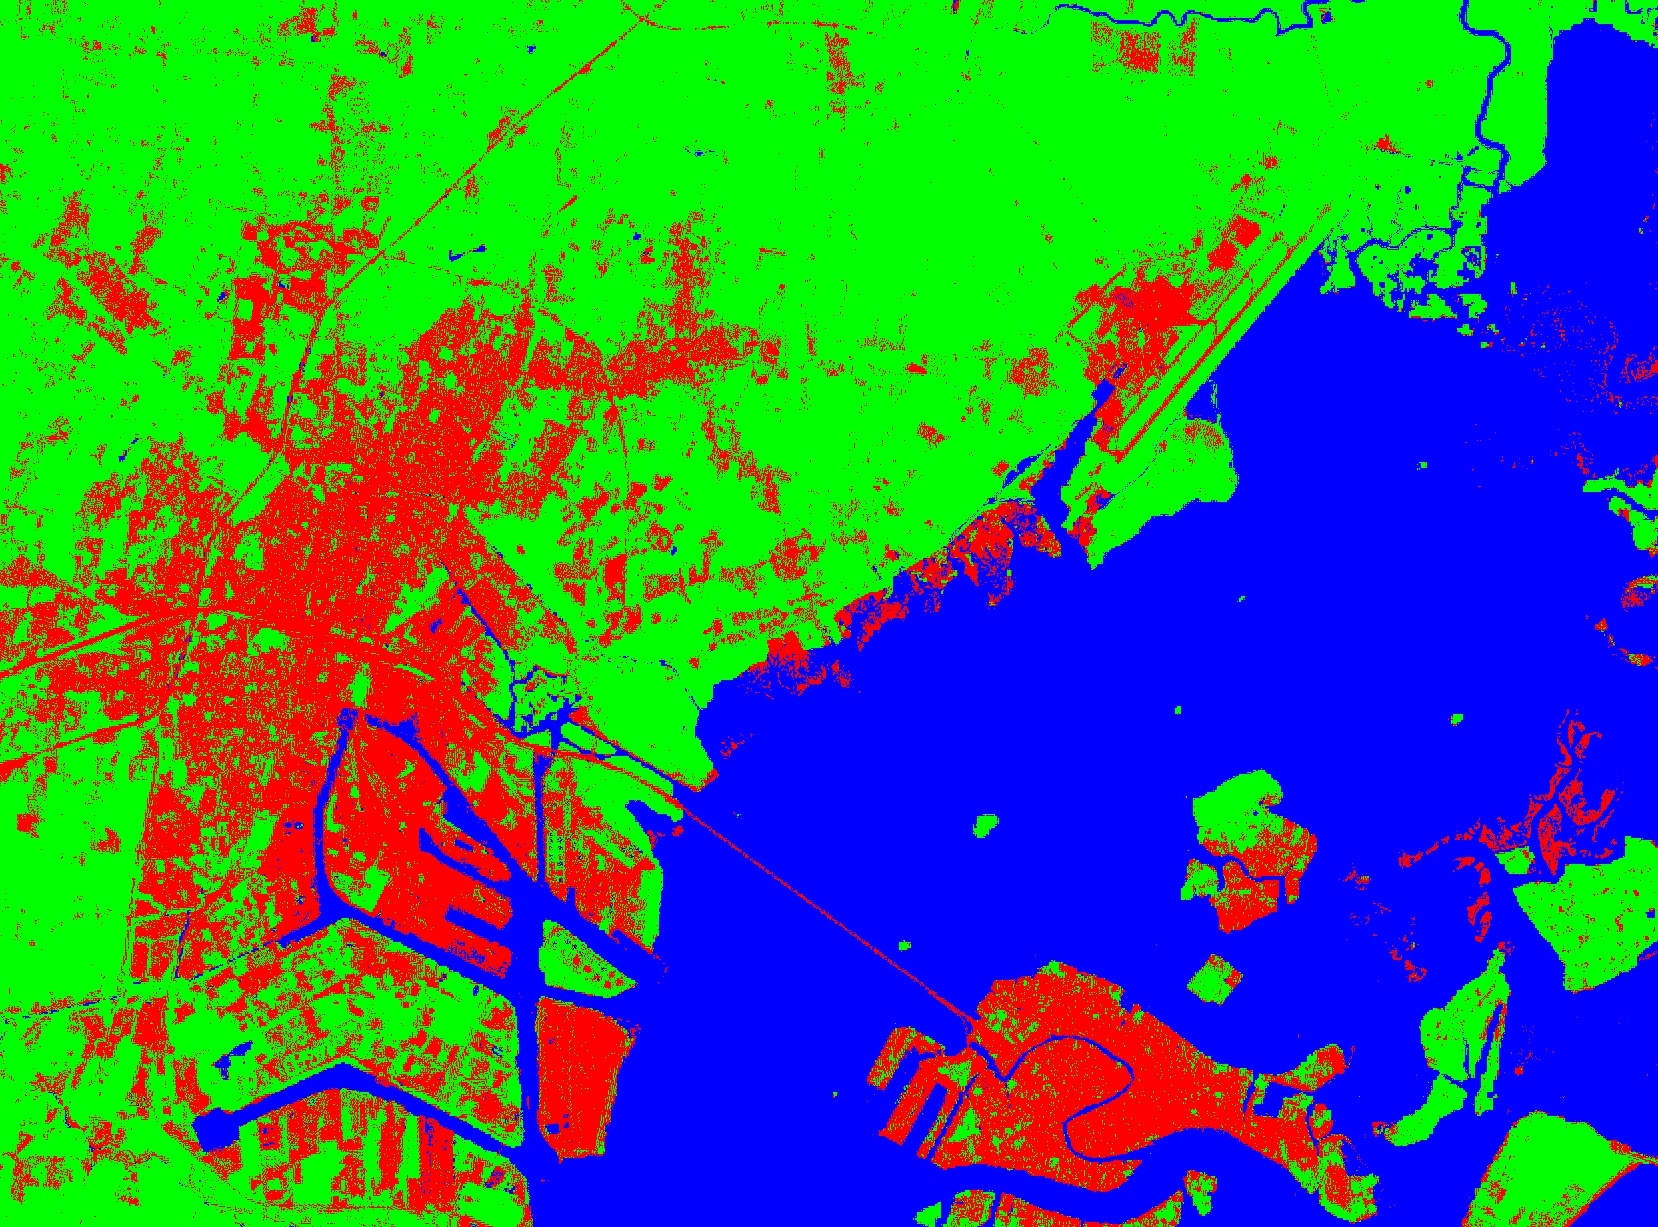
\includegraphics[height=250px]{LSE.png}
  \end{center}
\end{figure*}

\begin{figure*}
\begin{center}
  \caption{Superposition de l'image originale (en niveaux de gris) et de la classification des moindres carrés.}
  \label{veniseLSE}
  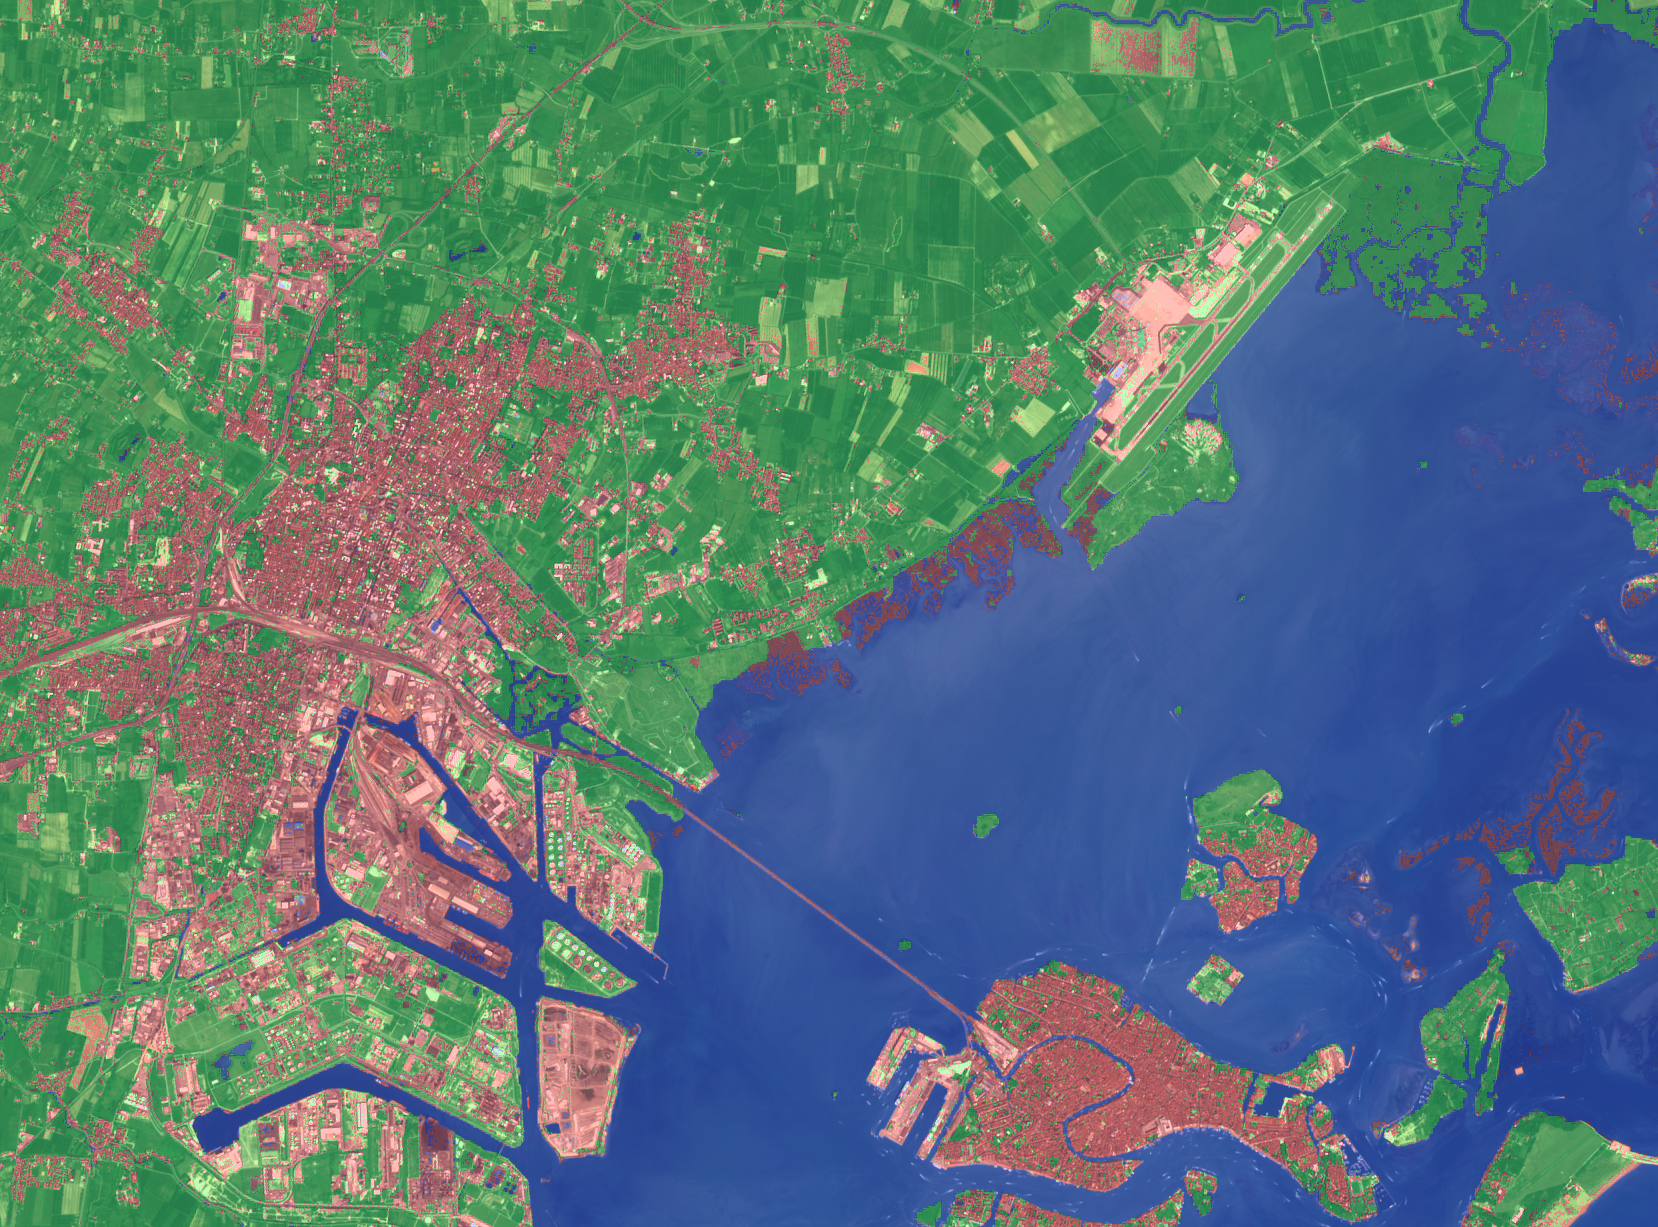
\includegraphics[height=250px]{veniseLSE.png}
  \end{center}
\end{figure*}

\begin{figure*}
\begin{center}
  \caption{Superposition de l'image originale (en niveaux de gris) et de la classification LDA.}
  \label{veniseLDA}
  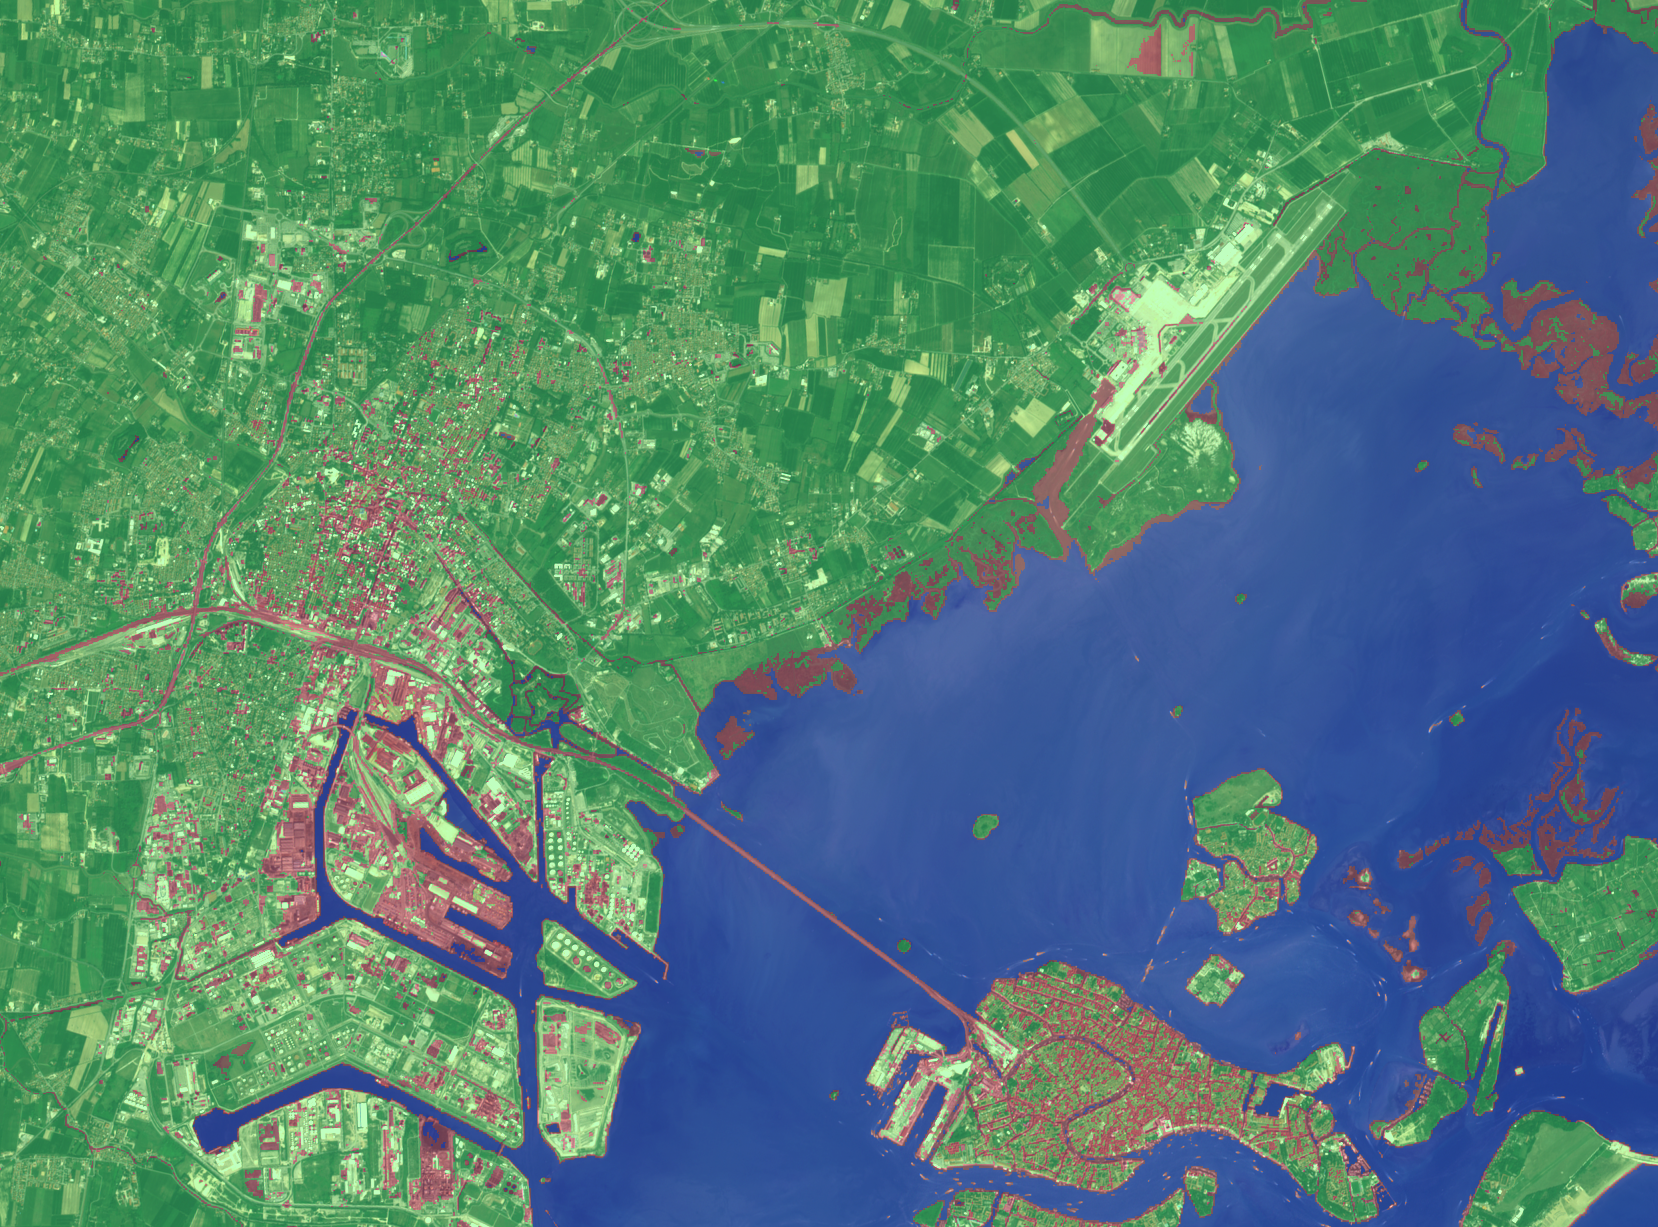
\includegraphics[height=250px]{veniseLDA.png}
  \end{center}
\end{figure*}

\begin{figure*}
\begin{center}
  \caption{Superposition de l'image originale (en niveaux de gris) et de la classification SVM.}
  \label{veniseSVM}
  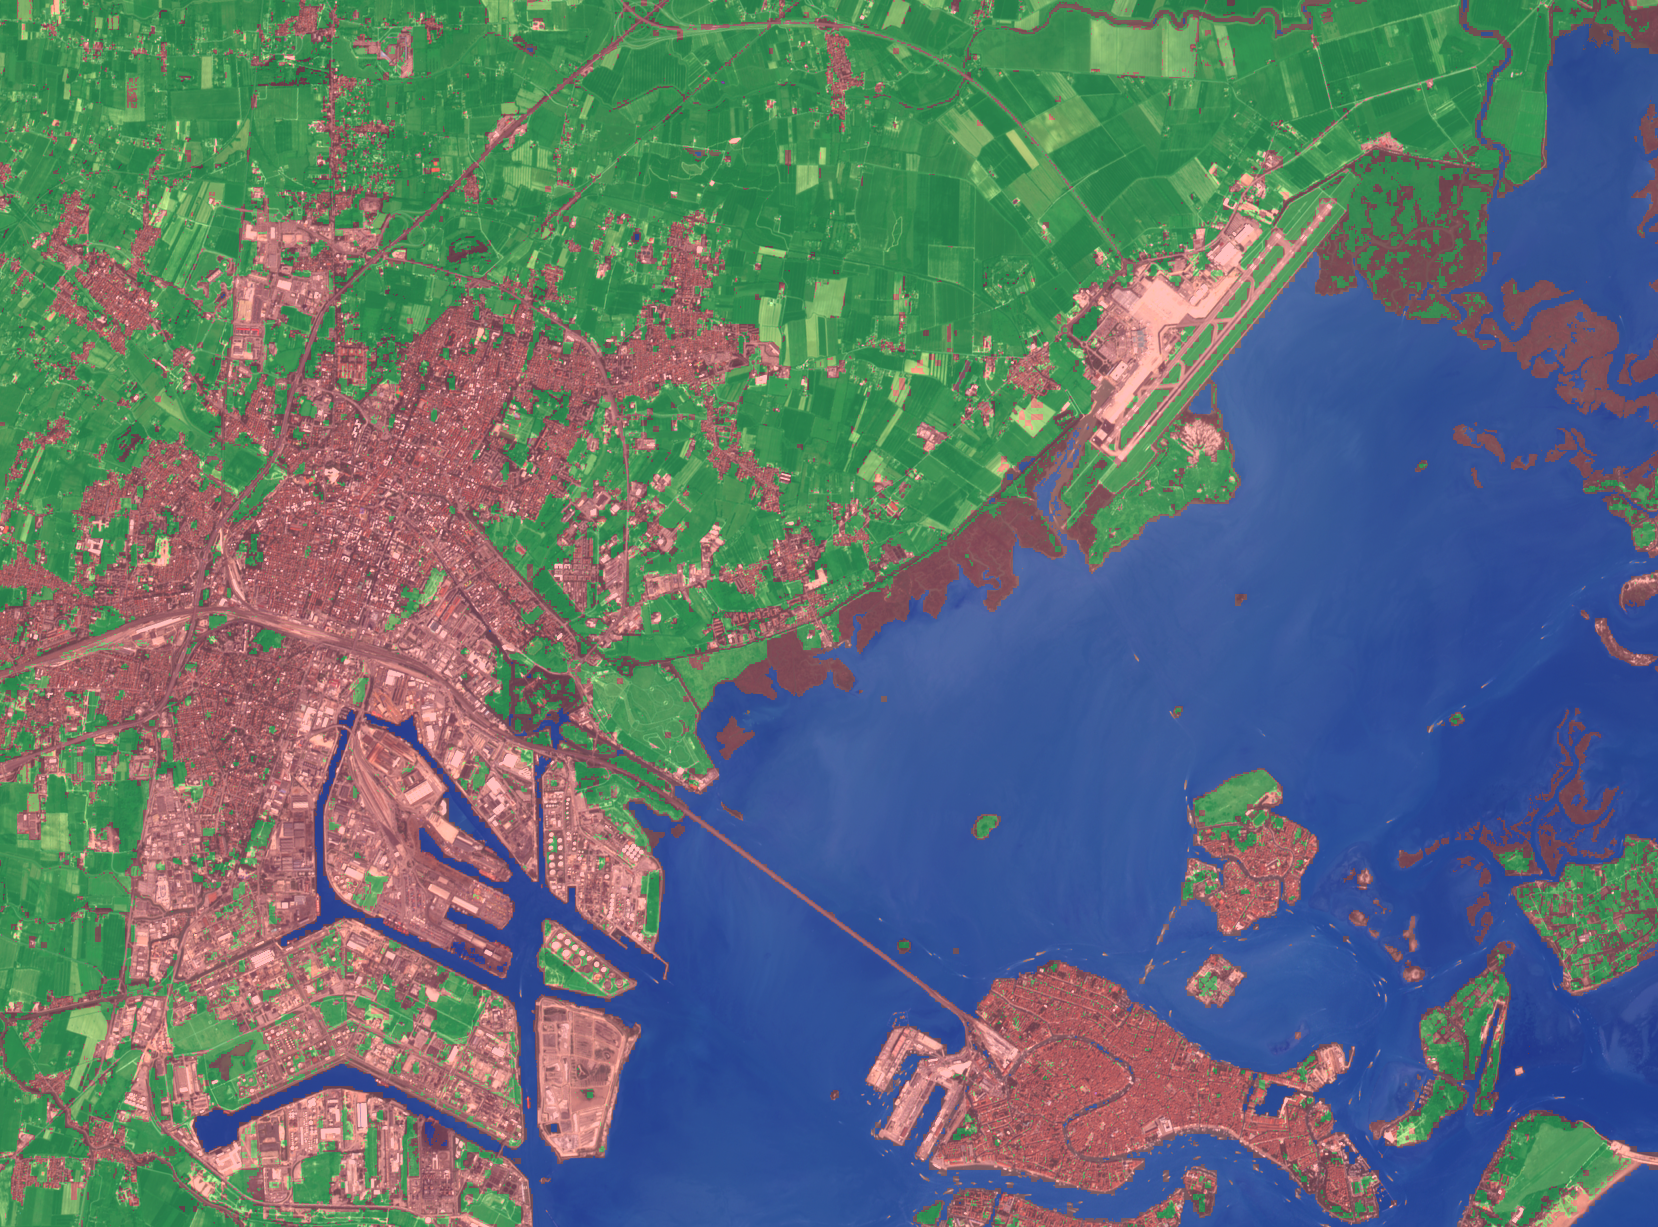
\includegraphics[height=250px]{veniseSVM.png}
  \end{center}
\end{figure*}
